\documentclass{beamer}
%
% Choose how your presentation looks.
%
% For more themes, color themes and font themes, see:
% http://deic.uab.es/~iblanes/beamer_gallery/index_by_theme.html
%
\mode<presentation>
{
  \usetheme{Madrid}      % or try Darmstadt, Madrid, Warsaw, ...
  \usecolortheme{default} % or try albatross, beaver, crane, ...
  \usefonttheme{default}  % or try serif, structurebold, ...
  \setbeamertemplate{navigation symbols}{}
  \setbeamertemplate{caption}[numbered]
} 

\usepackage[english]{babel}
\usepackage[utf8x]{inputenc}
\usepackage{hyperref}
\hypersetup{
    colorlinks = True,
    linkbordercolor = {white}
}

\title[ISU-01-06]{Processing ddRAD for population history inference}
\author{April Wright}
\institute{ISU and KU}
\date{01-06-2016}

\begin{document}

\begin{frame}
  \titlepage
\end{frame}

% Uncomment these lines for an automatically generated outline.
%\begin{frame}{Outline}
%  \tableofcontents
%\end{frame}

\section{Introduction}

\begin{frame}{Introduction}

\frametitle{ddRAD data}
\begin{itemize}
\item Reduced-representation genomic method
\end{itemize}
\end{frame}

\begin{frame}
\frametitle{ddRAD data}
\begin{itemize}
\item Reduced-representation genomic method
\item Cheap
\end{itemize}
\end{frame}

\begin{frame}
\frametitle{ddRAD data}
\begin{itemize}
\item Reduced-representation genomic method
\item Cheap
\item Lots of data returned
\end{itemize}
\end{frame}

\begin{frame}
\frametitle{ddRAD data}
\begin{itemize}
\item Reduced-representation genomic method
\item Cheap
\item Lots of data returned
\item Stable software pipelines for using these data
\end{itemize}
\end{frame}

\begin{frame}
\frametitle{A Quick Note}
Slides that contain ddRAD specific info will be noted. Some steps can be used with multiple data sources.
\end{frame}

\begin{frame}
\frametitle{Our Study}
\begin{block}{The Edwards Plateau}
% Your image included here
\begin{figure}
    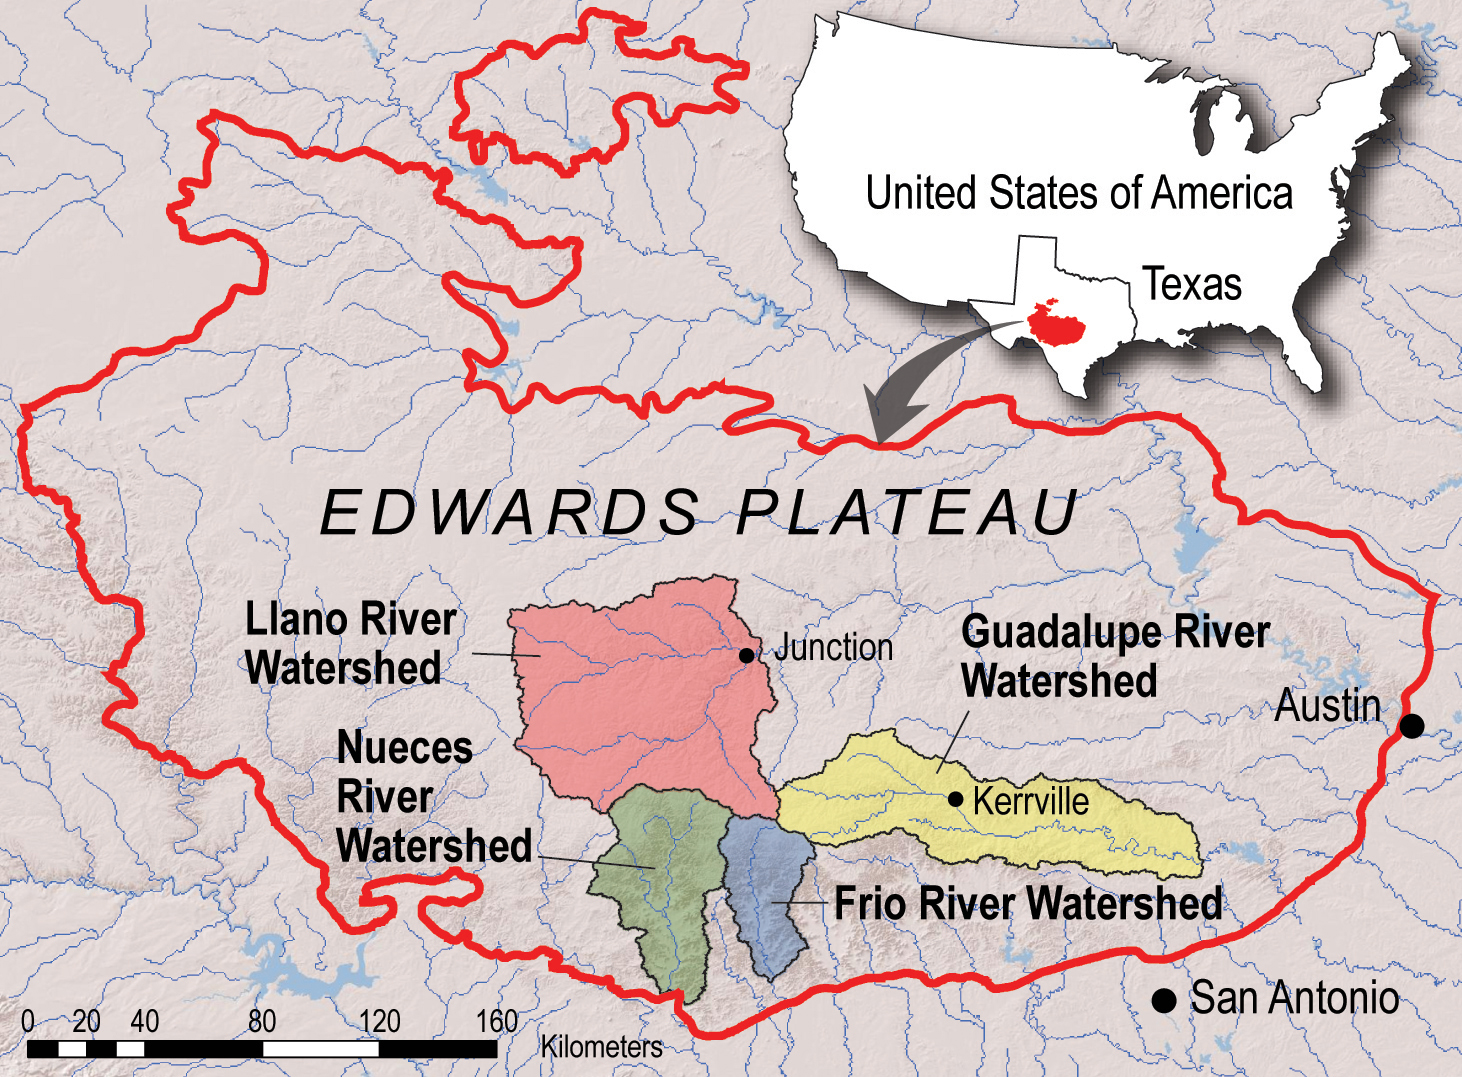
\includegraphics[scale=0.15]{pr_2010-06_map_hi-res.jpg}
    \caption{Image: AGU}
    \end{figure}
    \end{block}
\end{frame}

\begin{frame}
\frametitle{Our Study}
\begin{figure}
    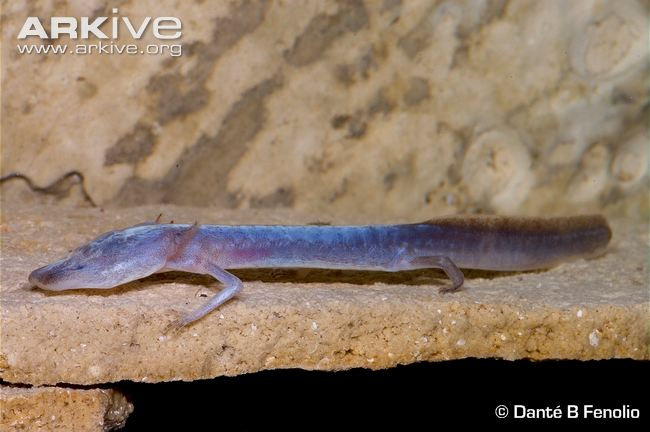
\includegraphics[scale=0.65]{Long-shot-of-Austin-blind-salamander.jpg}
	\caption{Arkive}
    \end{figure}
\end{frame}

\begin{frame}
\frametitle{Our Study}
13 putative species of \textit{Eurycea}
\end{frame}

\begin{frame}
\frametitle{Our Study}
13 putative species of \textit{Eurycea} \\
All of which are fairly threatened by development
\end{frame}

\begin{frame}
\frametitle{Our Study}
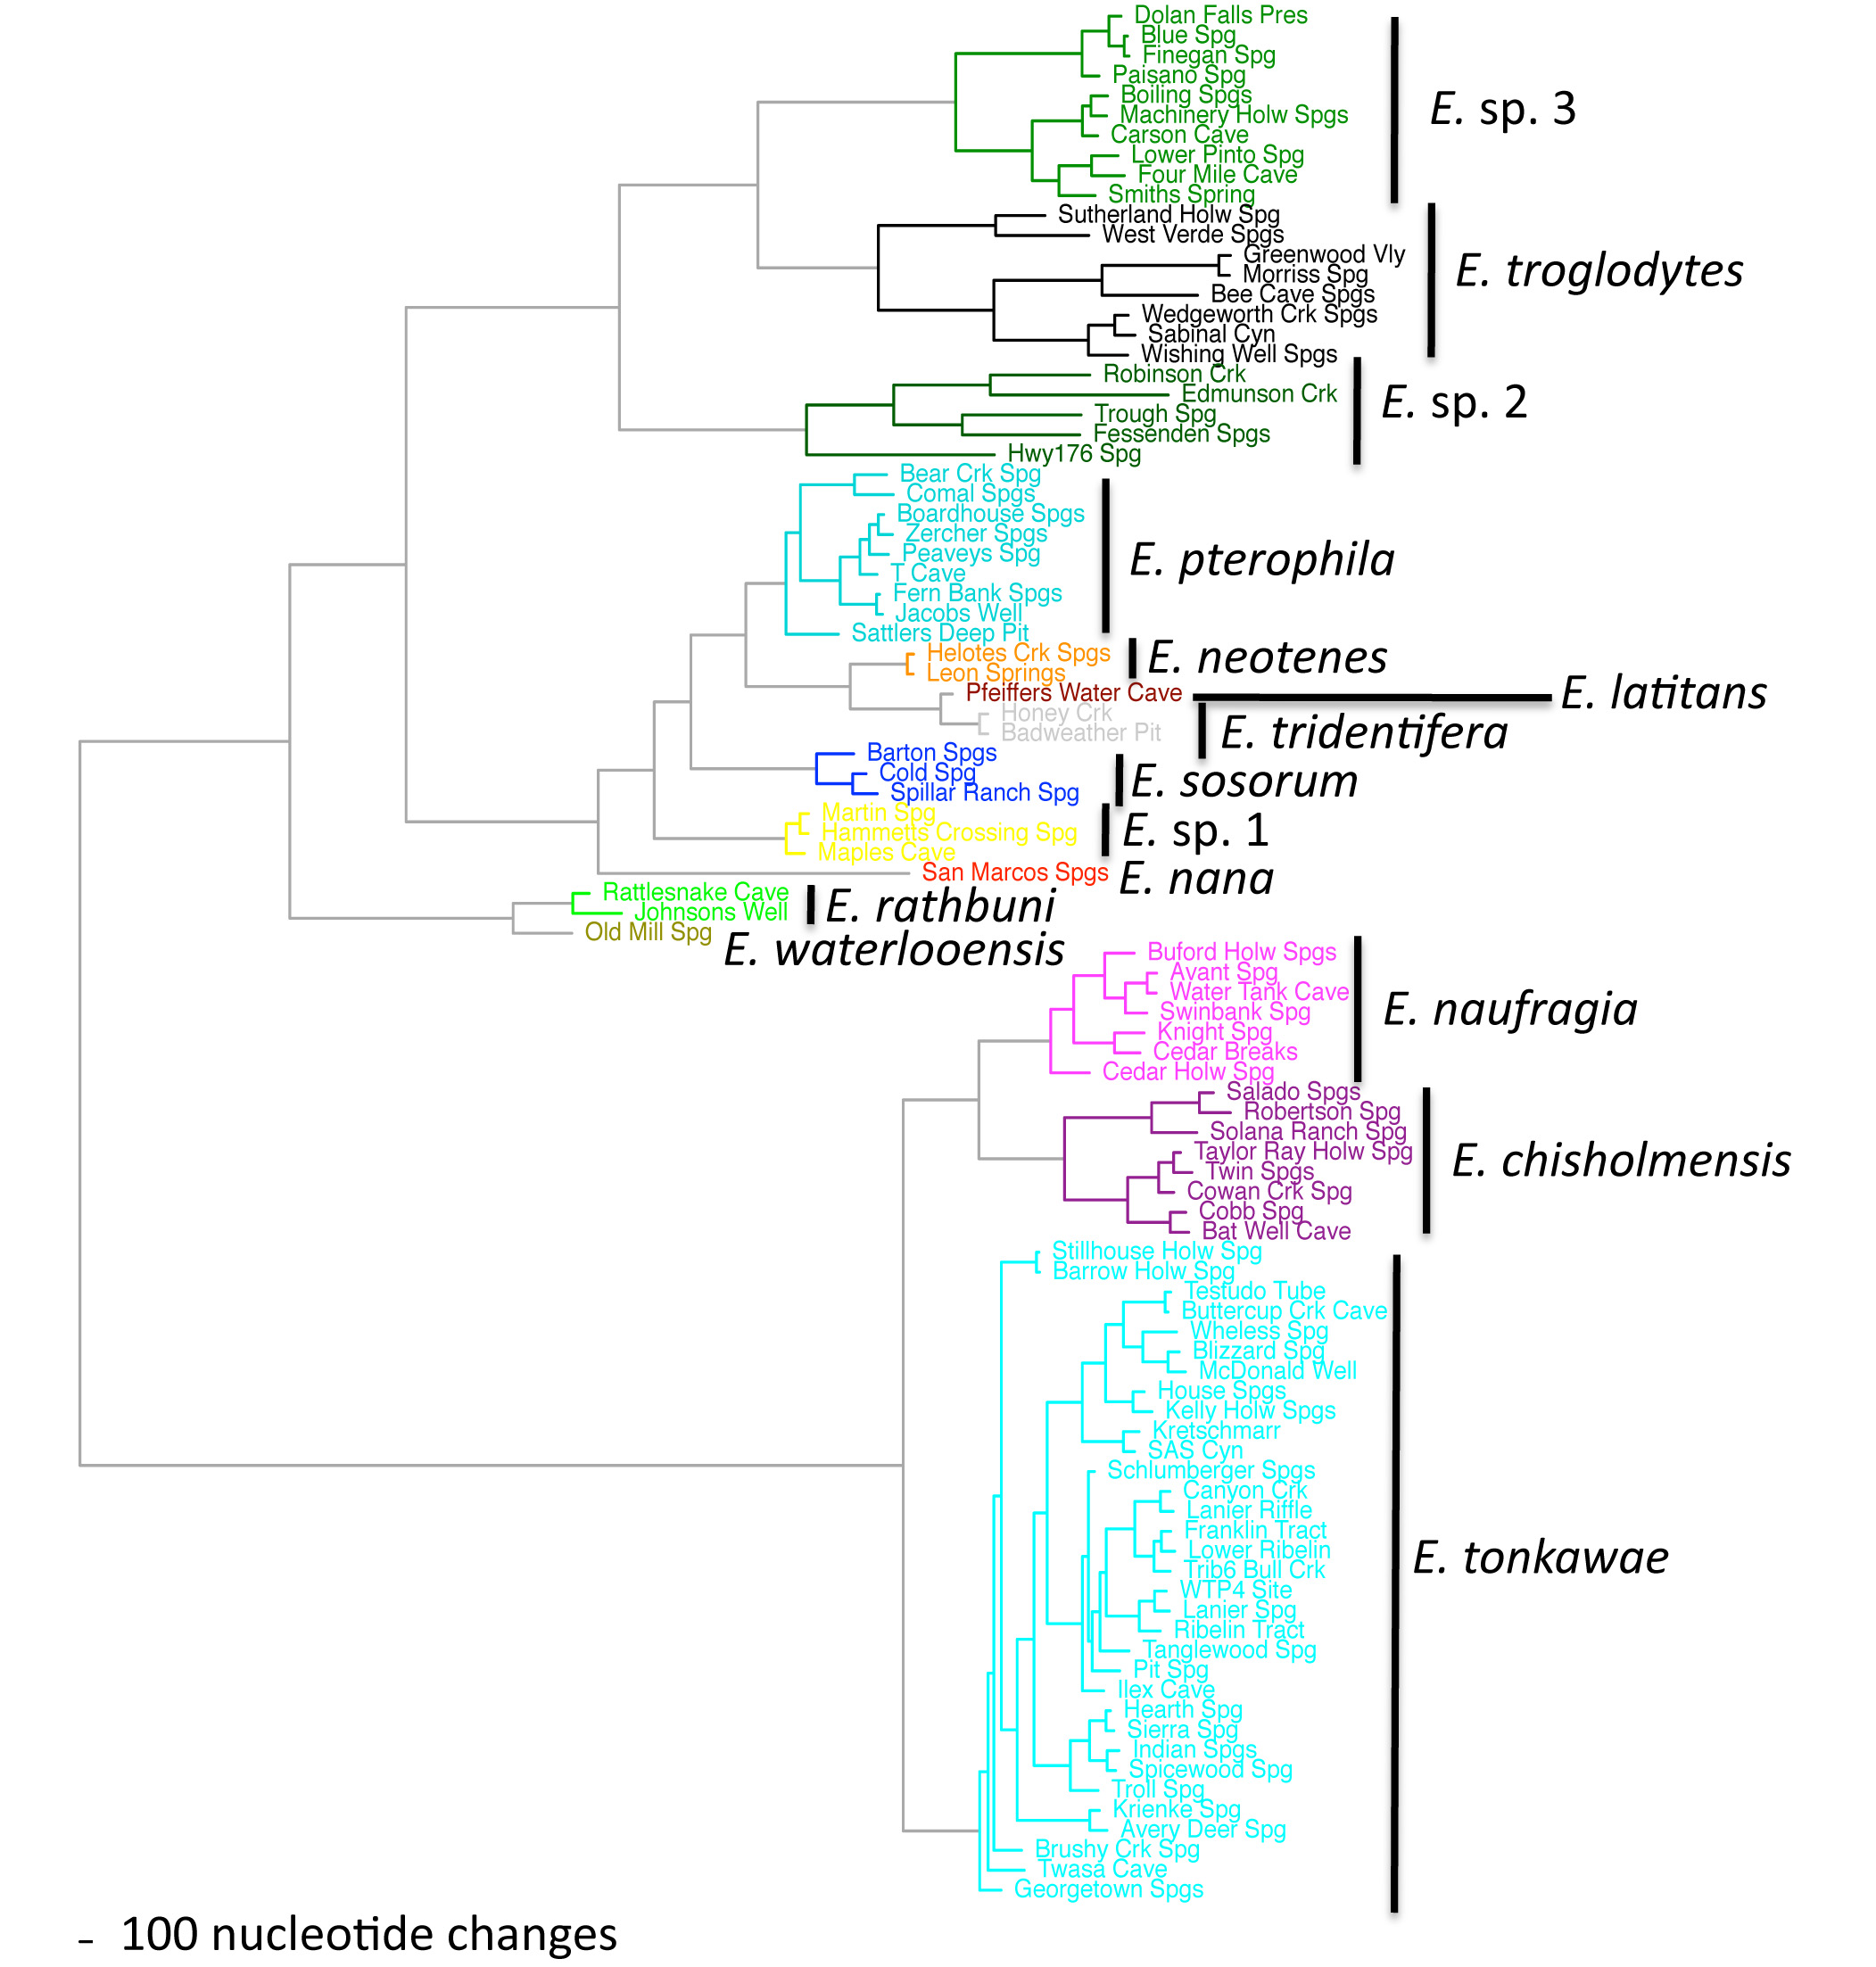
\includegraphics[scale=0.5]{PrelimTree.jpg}
\end{frame}

\begin{frame}
\frametitle{Our Study}
How many species of \textit{Eurycea} are there, really? \\
\end{frame}

\begin{frame}
\frametitle{Our Study}
How many species of \textit{Eurycea} are there, really? \\
And is there introgression between them?
\end{frame}

\begin{frame}
\frametitle{Our Study}
    \includegraphics[scale=0.75]{distro.jpg}

\end{frame}


\begin{frame}
\frametitle{Phylogenetics}
\begin{figure}
    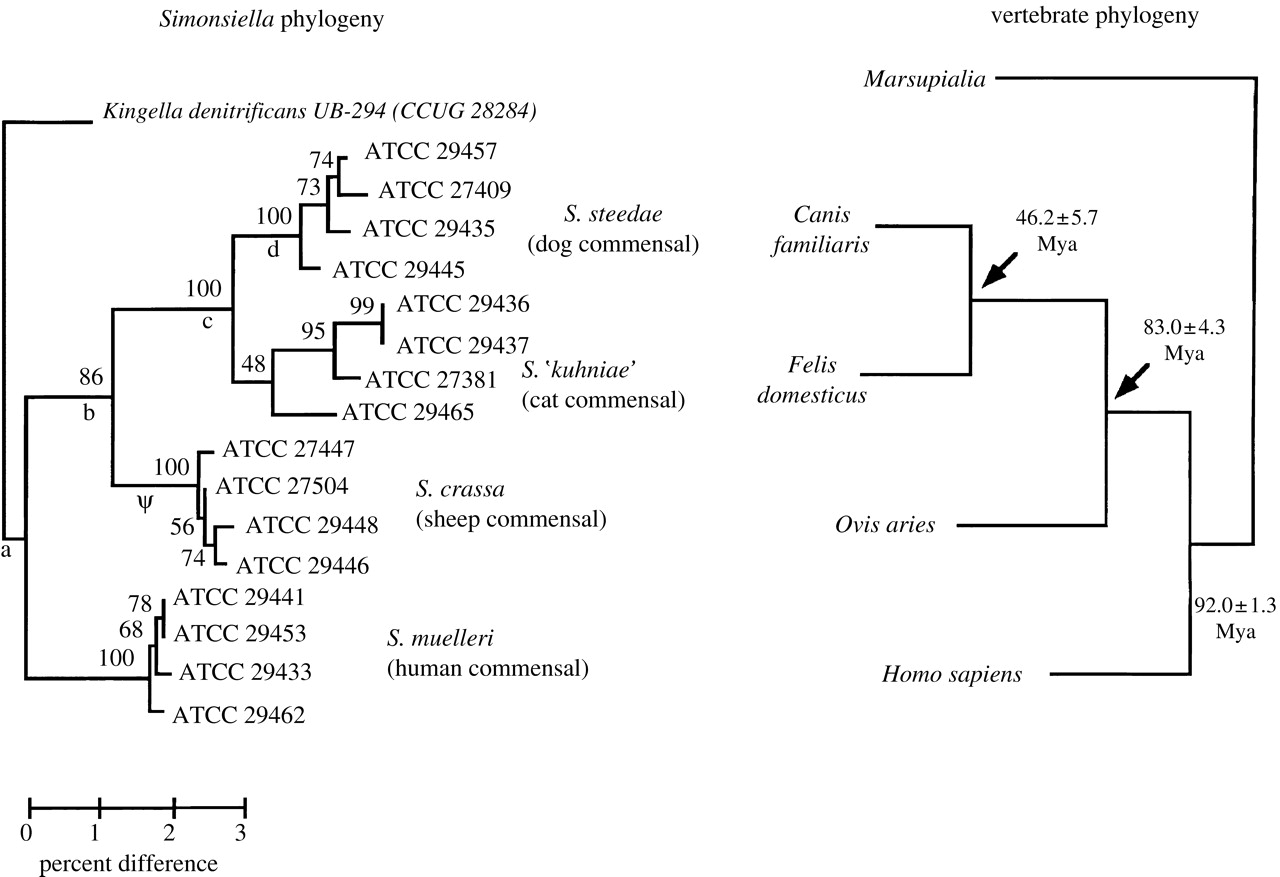
\includegraphics[scale=0.25]{F2_large.jpg}
	\caption{JP Staley, 2006. Figure 2}
    \end{figure}
\end{frame}


\begin{frame}
\frametitle{Phylogenetics}
\textbf{Maximum likelihood}
\end{frame}
\begin{frame}
\frametitle{Phylogenetics}
\textbf{Maximum likelihood} is a framework for estimating phylogeny by modeling the process of evolution that generated our sequence data
\end{frame}

\begin{frame}
\frametitle{Phylogenetics}
\begin{itemize}
\item \textbf{Maximum likelihood} is a framework for estimating phylogeny by modeling the process of evolution that generated our sequence data
\item Model-based 
\end{itemize}
\end{frame} 

\begin{frame}
\frametitle{Phylogenetics}
\begin{itemize}
\item \textbf{Maximum likelihood}is a framework for estimating phylogeny by modeling the process of evolution that generated our sequence data
\item Model-based: We make mathematically explicit assumptions 
\end{itemize}
\end{frame} 

\begin{frame}
\frametitle{Phylogenetics}
\begin{itemize}
\item \textbf{Maximum likelihood} is a framework for estimating phylogeny by modeling the process of evolution that generated our sequence data
\item Model-based: We make mathematically explicit assumptions 
\item Statistically consistent
\end{itemize}
\end{frame}

\begin{frame}
\frametitle{Phylogenetics}
\begin{itemize}
\item \textbf{Maximum likelihood} is a framework for estimating phylogeny by modeling the process of evolution that generated our sequence data
\item Model-based: We make mathematically explicit assumptions 
\item Statistically consistent: When we use the true model to analyze our data, we will eventually converge to the true answer as more data is added
\end{itemize}
\end{frame}
\begin{frame}
\frametitle{Phylogenetics}
\begin{itemize}
\item \textbf{Maximum likelihood} is a framework for estimating phylogeny by modeling the process of evolution that generated our sequence data
\item Model-based: We make mathematically explicit assumptions 
\item Statistically consistent: When we use the true model to analyze our data, we will eventually converge to the true answer as more data is added
\begin{itemize}
\item And because we are making mathematically-defined assumptions, we can use model-fitting to find the "true" model
\end{itemize}
\end{itemize}
\end{frame}

\begin{frame}
\frametitle{Phylogenetics}
\begin{itemize}
\item \textbf{Maximum likelihood} is a framework for estimating phylogeny by modeling the process of evolution that generated our sequence data
\item Model-based: We make mathematically explicit assumptions 
\item Statistically consistent: When we use the true model to analyze our data, we will eventually converge to the true answer as more data is added
\begin{itemize}
\item And because we are making mathematically-defined assumptions, we can use model-fitting to find the "true" model
\end{itemize}
\item Superimposed changes
\end{itemize}
\end{frame}


\begin{frame}
\frametitle{Phylogenetics}
\begin{itemize}
\item \textbf{Maximum likelihood} is a framework for estimating phylogeny by modeling the process of evolution that generated our sequence data
\item Model-based: We make mathematically explicit assumptions 
\item Statistically consistent: When we use the true model to analyze our data, we will eventually converge to the true answer as more data is added
\begin{itemize}
\item And because we are making mathematically-defined assumptions, we can use model-fitting to find the "true" model
\end{itemize}
\item Superimposed changes
\end{itemize}
\end{frame}

\begin{frame}
\frametitle{Phylogenetics}
\begin{itemize}
\item \textbf{Problems}
\end{itemize}
\end{frame}

\begin{frame}
\frametitle{Phylogenetics}
\begin{itemize}
\item \textbf{Problems}
\item Missing data
\end{itemize}
\end{frame}

\begin{frame}
\frametitle{Phylogenetics}
\begin{itemize}
\item \textbf{Problems}
\item \textbf{Biased} Missing data
\end{itemize}
\begin{figure}
    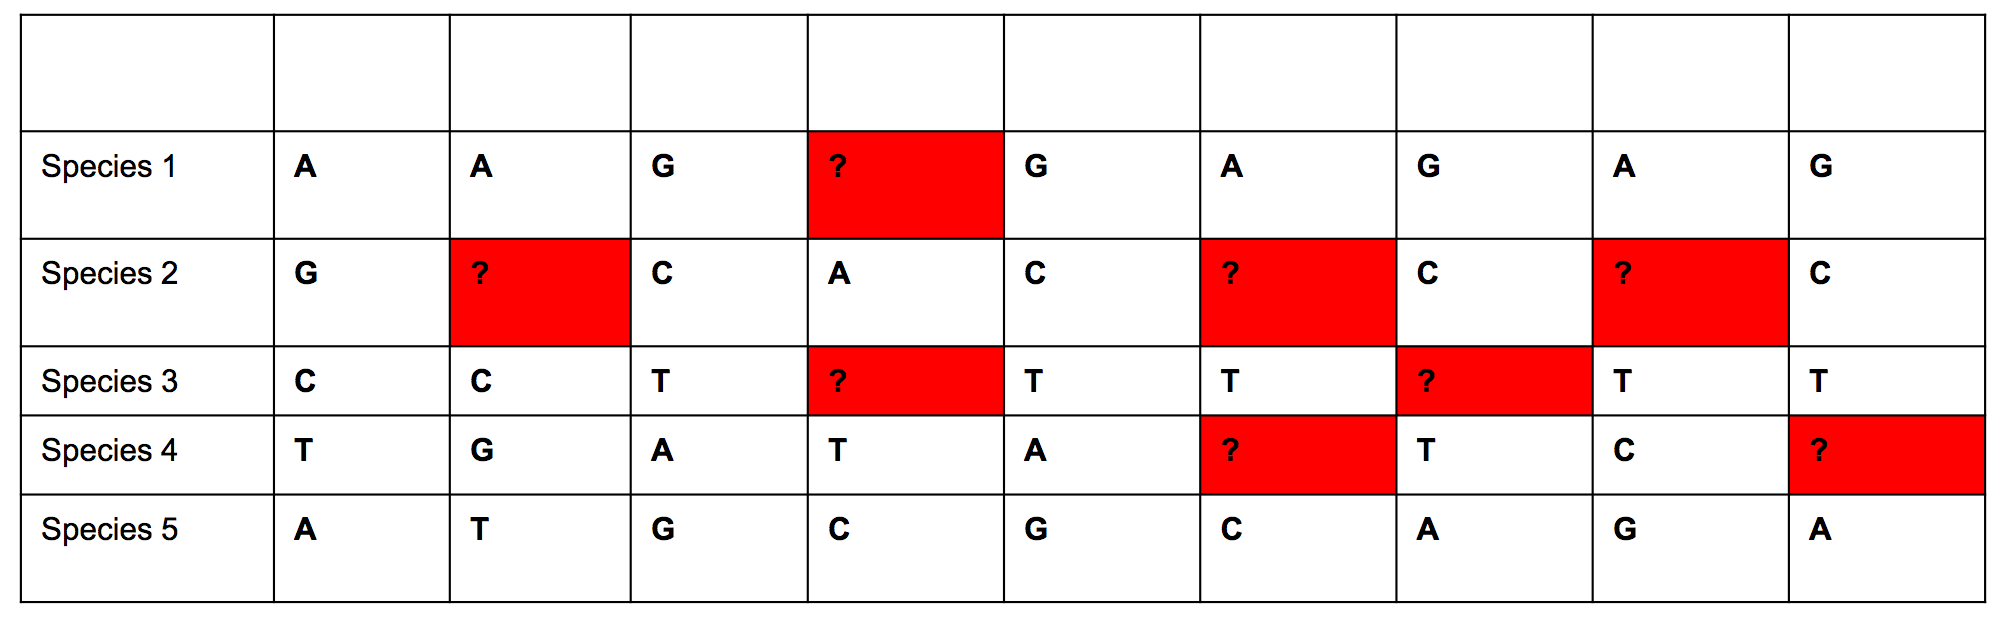
\includegraphics[scale=0.25]{Rando.png}
    \end{figure}
\end{frame}

\begin{frame}
\frametitle{Phylogenetics}
\begin{itemize}
\item \textbf{Problems}
\item \textbf{Biased} Missing data

\end{itemize}
\end{frame}



\begin{frame}
\frametitle{Phylogenetics}
\begin{itemize}
\item Missing data concentrated in specific individuals
\end{itemize}
\begin{figure}
    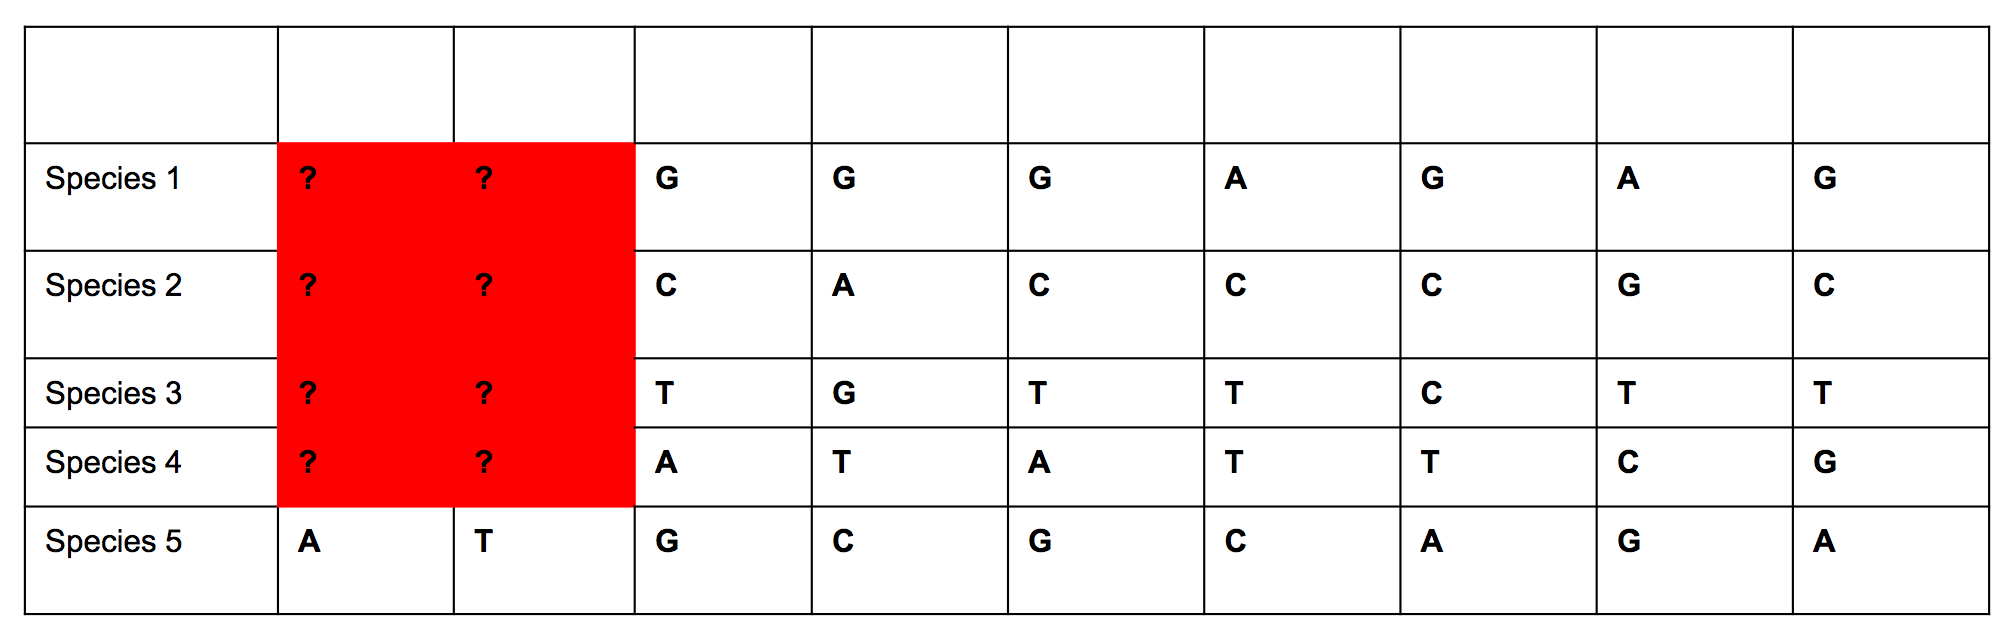
\includegraphics[scale=0.25]{individualized.png}
    \end{figure}
\end{frame}

\begin{frame}
\frametitle{Phylogenetics}
\begin{itemize}
\item Missing data concentrated in specific individuals
\item Missing data concentrated in certain loci in your data matrix
\end{itemize}
\begin{figure}
    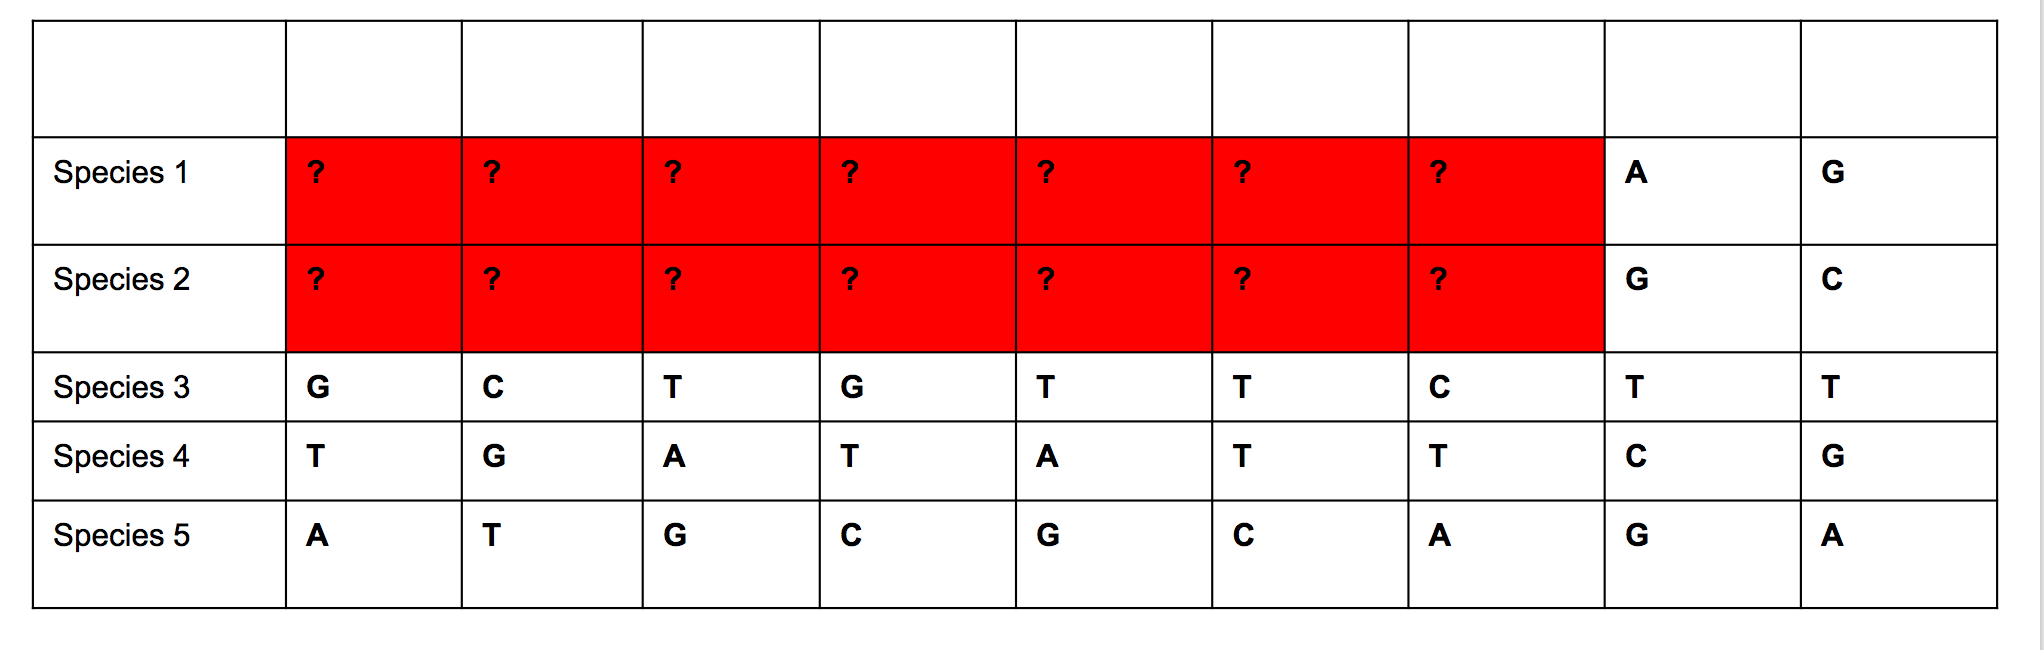
\includegraphics[scale=0.25]{bysite.png}
    \end{figure}
\end{frame}

\begin{frame}
\frametitle{Phylogenetics}
\begin{itemize}
\item \textbf{Problems}
\item Model misspecification

\end{itemize}
\end{frame}

\begin{frame}
\frametitle{Phylogenetics}
\begin{itemize}
\item \textbf{Problems}
\item Model misspecification: when your data are not adequately described by your model
\end{itemize}
\end{frame}

\begin{frame}
\frametitle{Phylogenetics}
Today, we'll be visualizing our data at every step to try and minimize a bias in which individuals have missing data
\end{frame}

\begin{frame}
\frametitle{Phylogenetics}
We'll also look at ways to make sure we aren't overly-conservative in our choosing of SNPs (i.e., biasing our collection towards sites that exhibit little change)
\end{frame}

\begin{frame}
\frametitle{The Demultiplex}
One of the things that makes RADseq, and especially ddRADseq, so cheap is the pooling of samples
\end{frame}

\begin{frame}
\frametitle{The Demultiplex}
One of the things that makes RADseq, and especially ddRADseq, so cheap is the pooling of samples \\
The way we recover individual samples is via demultiplexing
\end{frame}

\begin{frame}
\frametitle{The Demultiplex}
This allows for the cost-saving properties of batching, without the cost-increasing properties of synthesizing oligonucleotides. 
\end{frame}

\begin{frame}
\frametitle{The Demultiplex}
The STACKS step for this is called \href{http://catchenlab.life.illinois.edu/stacks/comp/process_radtags.php}{Process RAD Tags} 
\end{frame}

\begin{frame}
\frametitle{The Demultiplex}
Let's look at the output
\end{frame}

\begin{frame}
\frametitle{The Demultiplex}
Let's look at the output
\begin{itemize}
\item FASTQ files
\end{itemize}
\end{frame}

\begin{frame}
\frametitle{The Demultiplex}
Let's look at the output
\begin{itemize}
\item FASTQ files
\item Reads, grouped by individual
\end{itemize}
\end{frame}

\begin{frame}
\frametitle{The Demultiplex}
Let's look at the output
\begin{itemize}
\item FASTQ files
\item Reads, grouped by individual
\item We haven't done any SNP calling. This is just the step that gets our data ready to do that
\end{itemize}
\end{frame}

\begin{frame}
\frametitle{Initial Identification of SNPs}
For this step, we will use \href{http://catchenlab.life.illinois.edu/stacks/comp/ustacks.php}{ustacks}
\end{frame}

\begin{frame}
\frametitle{Initial Identification of SNPs}
Each RAD tag has usually been sequenced multiply per-individual
\end{frame}

\begin{frame}
\frametitle{Initial Identification of SNPs}
Each RAD tag has usually been sequenced multiply per-individual \\
This allows us to sort tags into "stacks" of identical and unique reads
\end{frame}

\begin{frame}
\frametitle{Initial Identification of SNPs}
Each RAD tag has usually been sequenced multiply per-individual \\
This allows us to sort tags into "stacks" of identical and unique reads
From these sets of identical and unique reads, we do a first pass at identifying SNPs.
\end{frame}

\begin{frame}
\frametitle{Initial Identification of SNPs}
\textbf{Key Parameters}
\begin{itemize}
\item -m: Minimum depth of coverage
\item -M: Maximum mismatches allowed between reads in a stack
\end{itemize}
\end{frame}

\begin{frame}
\frametitle{Initial Identification of SNPs}
\textbf{Other Parameters}
\begin{itemize}
\item -i: ID for this sample
\end{itemize}
\end{frame}

\begin{frame}
\frametitle{Exercise}
I've included a script, countSNPs.sh, and another, plotPutativeSNPs.py
\end{frame}

\begin{frame}
\frametitle{Exercise}
One of the issues we discussed was biased missing data
\end{frame}

\begin{frame}
\frametitle{Catalog Building}
Once we have our within-individual stacks, we build a catalog of loci across individual catalogs (\href{http://catchenlab.life.illinois.edu/stacks/comp/cstacks.php}{cstacks})
\end{frame}

\begin{frame}
\frametitle{Catalog Building}
\textbf{Key Parameters}
\begin{itemize}
\item -m: Maintain tags that match more than one RAD tag
\item -n: number of mismatches to allow between a putative tag, and a tag in the catalog
\end{itemize}
\end{frame}

\begin{frame}
\frametitle{Catalog Building}
\textbf{Exercise}
\begin{itemize}
\item cstacks.sh
\item Choose a different value for -n
\end{itemize}
\end{frame}

\begin{frame}
\frametitle{Catalog Building}
\textbf{Exercise}
\begin{itemize}
\item How many lines (SNPs) are in this catalog?
\end{itemize}
\end{frame}

\begin{frame}
\frametitle{Check Individuals Against Catalog}
We use \href{http://catchenlab.life.illinois.edu/stacks/comp/sstacks.php}{sstacks} for this
\end{frame}
\begin{frame}
\frametitle{Catalog Building}
\textbf{Exercise}
\begin{itemize}
\item Run sstacks
\item Use countMatches.sh and plotMatches.py to see how many SNPs for each individual match the catalog
\end{itemize}
\end{frame}

\begin{frame}
\frametitle{Outputting Data for Phylogenetics}
We use \href{http://catchenlab.life.illinois.edu/stacks/comp/populations.php}{populations} for this. 
\end{frame}

\begin{frame}
\frametitle{Outputting Data for Phylogenetics}
A new file is needed, here: \textbf{the population map}
\end{frame}

\begin{frame}
\frametitle{Outputting Data for Phylogenetics}
\textbf{Key Parameters}
\begin{itemize}
\item -r: Percentage of individuals in a population that must have a locus to output it
\item -m: Minimum stack depth at a locus
\end{itemize}
\end{frame}

\begin{frame}
\frametitle{Exercise}
Looking at this output is easy.
\end{frame}

\begin{frame}
\frametitle{Exercise}
Looking at this output is easy.
But we can also look in a more complex way: countPhyloMissing.sh and plotPhyloMissing.py
\end{frame}

\begin{frame}
\frametitle{RAxML approximate likelihoods}

\begin{tabular}{ l  | r }
  323320 & -288336.664115  \\
  323340 & -84377.460743 \\
  323360 & -27407.770692\\
  323380 & -10281.525371\\
  323390 & -1699.210794 \\
\end{tabular}
\end{frame}

\begin{frame}
\frametitle{Lastly, let's build the tree}
RAxML Approximate final L scores

\end{frame}

\begin{frame}
\frametitle{Lastly, let's build the tree}
Garli
\end{frame}

\end{document}
